\subsection[\radar~\texttt{RADAR}]{\texorpdfstring{\radar Fighting Byzantine Contributions in Heterogeneous Settings}{Fighting Byzantine Contributions in Heterogeneous Settings}}



\begin{frame}{Handling Byzantine Contributions in Heterogeneous Settings}
  \stepcounter{beamerpauses}
  \begin{columns}
    \column{.5\textwidth}
    \textbf{Working assumptions}
    \begin{itemize}
      \item Multiple organizations using a FIDS.
      \item Partial heterogeneity in the datasets: different data distributions but existing similarities.
    \end{itemize}

    \onslide<+(1)->{
      \textbf{Byzantine contributions}
      \begin{itemize}[<+->]
        \item data quality issues (\eg, labelling, noise);
        \item distribution mismatches; and
        \item adversaries\alt<+->{, \alert{possibly colluding}.}{.}
      \end{itemize}
    }

    \column{.5\textwidth}
    \onslide<2->
    \begin{figure}
      \centering
      \includegraphics<1-4>[width=\textwidth]{figures/radar-eval/setup/partition.pdf}%
      \includegraphics<5->[width=\textwidth]{figures/radar-eval/setup/poisoning.pdf}%
    \end{figure}

  \end{columns}

\end{frame}

















\begin{frame}{Introducing \texttt{RADAR}}
  \centering
  \begin{figure}
    \centering
    \foreach \i in {1,...,4} {
      \includegraphics<\i>[width=.95\linewidth,left]{figures/thesis/radar/agenda/\i.pdf}%
    }
    \vspace{-2em}
    \caption{\texttt{RADAR}~\footcite{lavaur_radar_2024} architecture, combining \emph{subjective} clustering and reputation-weighted aggregation to mitigate the impact lower-quality contributions.}
    \label{fig:radar}
  \end{figure}
\end{frame}




















\newcommand{\hr}{\cellcolor{red!30}}
\newcommand{\ho}{\cellcolor{orange!30}}
\newcommand{\hg}{\cellcolor{green!30}}

\begin{frame}{Handling heterogeneity}
  \begin{columns}
    \begin{column}{.4\textwidth}
      \begin{figure}
        \captionsetup{justification=centering}
        \includegraphics<1>[width=\linewidth,left]{./figures/radar-eval/clustering/clustering_benign.pdf}%
        \caption{Clustering results without poisoning.\\
        Rand index=1.0}
      \end{figure}
    \end{column}
    \begin{column}{.6\textwidth}

      \begin{table}
        \centering
        \caption*{Accuracy for different baselines.}
        \footnotesize
        \setlength\tabcolsep{.5ex}
        \begin{tabularx}{.8\textwidth}{>{\raggedright\arraybackslash}p{2.15cm}|ccc}
          \toprule % ---------------------------------
          \textbf{Scenario}
          & \multicolumn{1}{c}{\texttt{RADAR}} & \multicolumn{1}{c}{\texttt{FoolsGold}} & \multicolumn{1}{c}{\texttt{Clustered}} \\
          \midrule % ---------------------------------
          \textbf{Benign} & \hg 99.07 & \hr 55.04 & \hg 99.24  \\
        \end{tabularx}
        \caption*{\footnotesize More is better}

      \end{table}
    \end{column}
  \end{columns}
\end{frame}

\begin{frame}{Handling Untargeted Byzantines}
  \begin{columns}
    \begin{column}{.4\textwidth}
      \begin{figure}
        \captionsetup{justification=centering}
        \only<1>{
          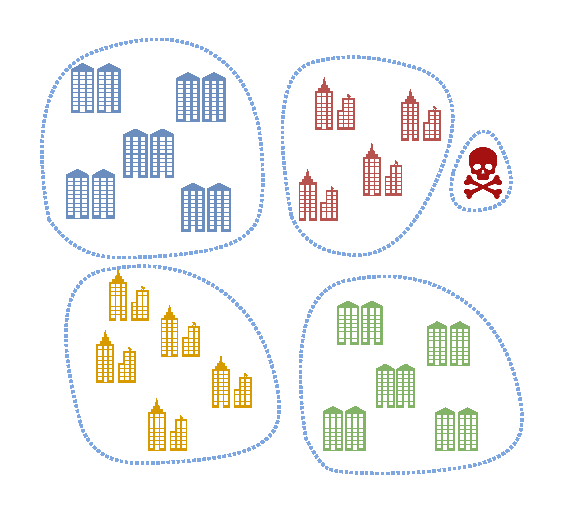
\includegraphics[width=\linewidth,left]{./figures/radar-eval/clustering/clustering_lone_untargeted.pdf}
          \caption*{Clustering results for\\
            \texttt{lone 100U}.\\
            Rand index=1.0
          }
        }
        \only<2>{
          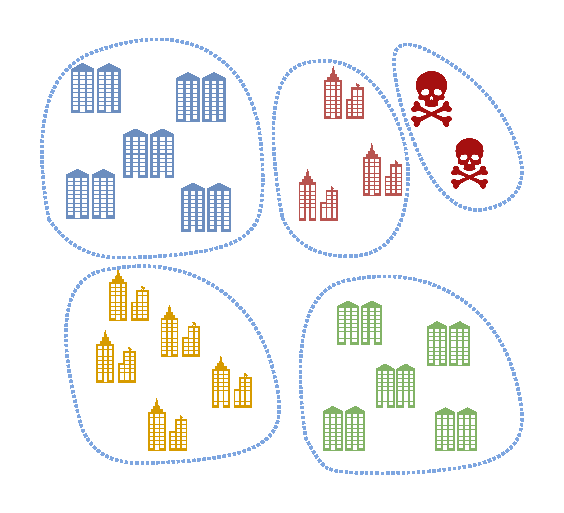
\includegraphics[width=\linewidth,left]{./figures/radar-eval/clustering/clustering_min_untargeted.pdf}
          \caption*{Clustering results for\\ \texttt{colluding minority 100U}\\
            Rand index=1.0
          }
        }
        \only<3>{
          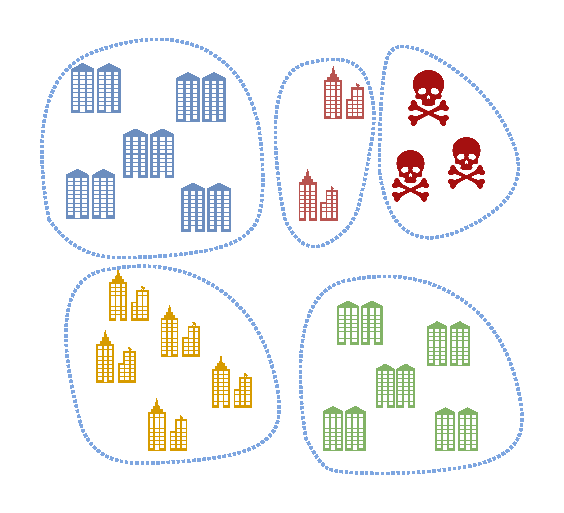
\includegraphics[width=\linewidth,left]{./figures/radar-eval/clustering/clustering_maj_untargeted.pdf}
          \caption*{Clustering results for\\
            \texttt{colluding majority 100U}\\
            Rand index=1.0
          }
        }
      \end{figure}
    \end{column}

    \begin{column}{.6\textwidth}
      \begin{table}
        \centering

        \footnotesize
        \setlength\tabcolsep{1ex}
        \caption*{Attack success rate for different baselines.}
        \begin{tabularx}{.9\textwidth}{l>{\raggedright\arraybackslash}p{2.15cm}ccc}
          \toprule % ---------------------------------
          \multicolumn{2}{c}{{\textbf{Scenario}}}
          & \multicolumn{1}{c}{\texttt{RADAR}} & \multicolumn{1}{c}{\texttt{FoolsGold}} & \multicolumn{1}{c}{\texttt{Clustered}} \\
          \midrule % ---------------------------------
          % % UNTARGETED ATTACKS
          \multicolumn{2}{l}{\textbf{Untargeted} (\texttt{100U})}  & & & \\
          & \texttt{Lone} & \hg 0.08 &\hr 99.89 & \hg 0.12 \\
          \only<2->{& \texttt{Collud.~min.} & \hg 0.10 & \hg 0.04 &\ho 6.26 \\}
          \only<3->{& \texttt{Collud.~maj.} & \hg 0.08 &\ho 38.98 & \hr 94.36 \\}
        \end{tabularx}
        \caption*{\footnotesize Less is better}
      \end{table}

    \end{column}
  \end{columns}
\end{frame}


\begin{frame}{Handling Targeted Byzantines}
  \begin{columns}
    \begin{column}{.4\textwidth}
      \begin{figure}
        \centering
        \captionsetup{justification=centering}
        \only<1-2>{%
          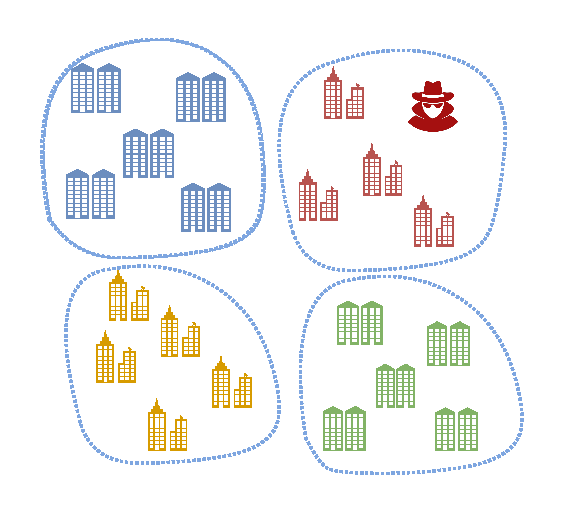
\includegraphics[width=\linewidth,left]{figures/radar-eval/clustering/clustering_lone_targeted.pdf}
          \caption*{
            Clustering results for\\
            \texttt{Lone 100T}\\
            Rand index=0.97
          }
        }
        \only<3>{%
          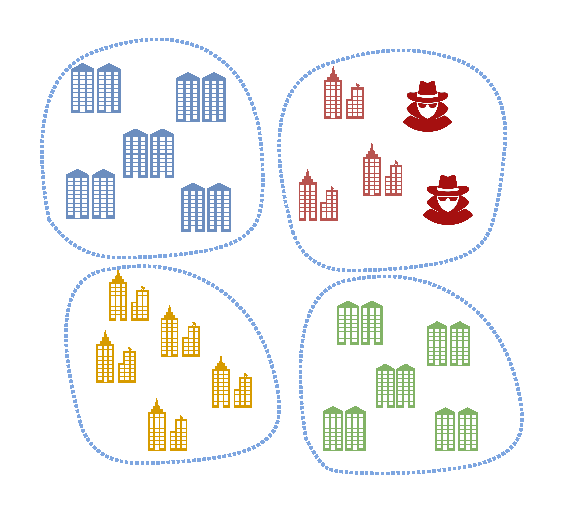
\includegraphics[width=\linewidth,left]{./figures/radar-eval/clustering/clustering_min_targeted.pdf}%
          \caption*{
            Clustering results for\\
            \texttt{colluding minority 100T}\\
            Rand index=0.97
          }
        }
        \only<4>{
          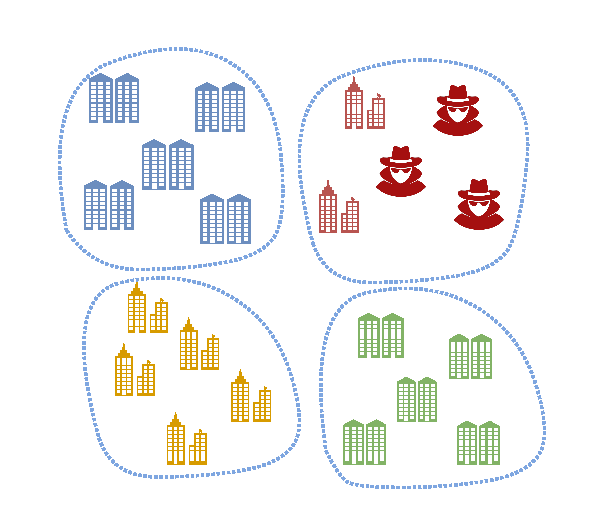
\includegraphics[width=\linewidth,left]{./figures/radar-eval/clustering/clustering_maj_targeted.pdf}%
          \caption*{Clustering results for \texttt{colluding majority 100T}\\
          Rand index=0.96}
        }

      \end{figure}
    \end{column}
    \begin{column}{.6\textwidth}
      \begin{table}
        \centering
        \footnotesize
        \setlength\tabcolsep{1ex}
        \caption*{Attack success rate for different baselines.}

        \begin{tabularx}{.9\textwidth}{l>{\raggedright\arraybackslash}p{2.15cm}ccc}
          \toprule % ---------------------------------
          \multicolumn{2}{c}{{\textbf{Scenario}}}
          & \multicolumn{1}{c}{\texttt{RADAR}} & \multicolumn{1}{c}{\texttt{FoolsGold}} & \multicolumn{1}{c}{\texttt{Clustered}} \\
          \midrule % ---------------------------------
          % % TARGETED ATTACKS
          \multicolumn{2}{l}{\textbf{Targeted} (\texttt{100T})}  & & & \\
          & \texttt{Lone} &\hg 0.00 & \hr 93.82 & \hg 0.45 \\
          \only<3->{& \texttt{Collud.~min.} & \hg 0.00 & \hg 2.97 & \hr 53.40 \\}
          \only<4->{& \texttt{Collud.~maj.} &  \hr 73.39 & \ho 8.10 & \hr 59.36 \\}
        \end{tabularx}

        \caption*{\footnotesize Less is better}
      \end{table}
      \vspace{-1em}

      \only<2>{
        \begin{minipage}{\textwidth}
          \begin{figure}
            \captionsetup{justification=centering}
            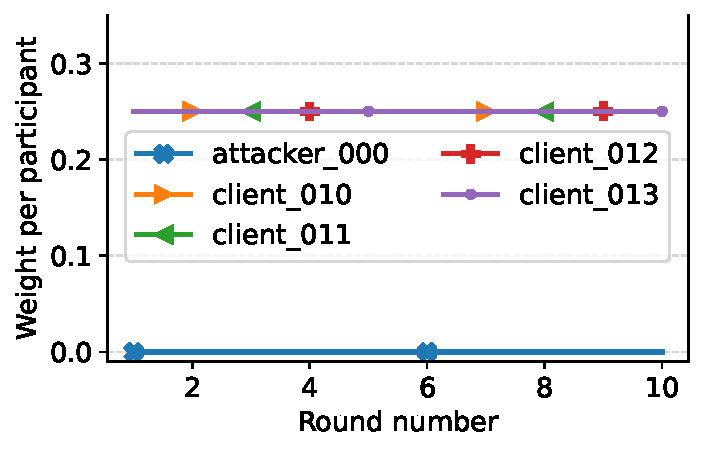
\includegraphics[width=.6\linewidth]{./figures/radar-eval/reput/lone_loud_expanded.pdf}
            \caption{Aggregation weights.}
          \end{figure}
      \end{minipage}}

      %   \only<5>{\begin{minipage}{\textwidth}
      %       \begin{figure}
      %           \captionsetup{justification=centering}
      %           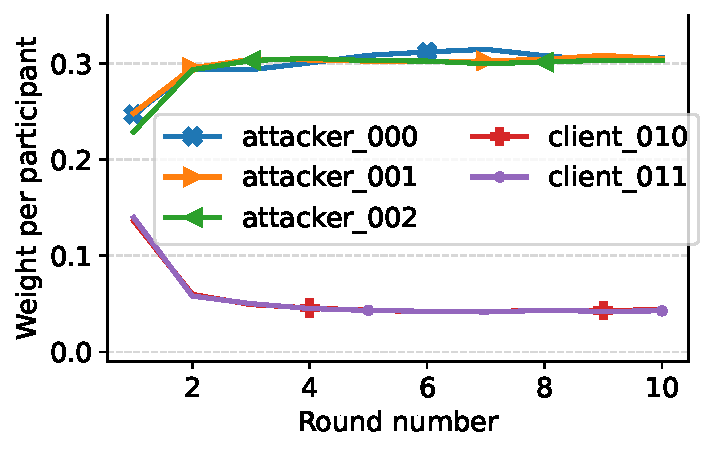
\includegraphics[width=.6\linewidth]{./figures/radar-eval/reput/byzantine_majority_loud_expanded.pdf}
      %           \caption{Aggregation weights.}
      %       \end{figure}
      %  \end{minipage}}

    \end{column}
  \end{columns}
\end{frame}

\begin{frame}{Highlights}
  \begin{block}{Combining clustering and mitigation strategy is effective}
    Clustering effectively creates \alert{homogeneous} communities where conventional mitigation can be applied.
  \end{block}

  \pause
  \begin{block}{Cross-evaluation enable \alert{true} reputation-aware FL}
    Only way to gather indirect feedbacks (\ie, one clients' evaluation of another's contribution); at the cost of scalability.
  \end{block}

  \pause
  \begin{block}{Generalizable outside intrusion detection}
    With a few conditions: parametric models, locally owned evaluation set, a \alert{small-scale use case}, and a \alert{trusted central server}.
  \end{block}
\end{frame}




